\begin{frame}[plain]
  \vfill
  \centering
  \Huge Multimodal Architectures
  \vfill
\end{frame}

\begin{frame}{Example Multimodal Architecture: Video Classification with Text, Audio, and Visual Streams}
  \begin{columns}
    \begin{column}{0.55\textwidth}
      \textbf{Multimodal video classification:}\\[0.6em]
      \begin{itemize}
        \item \textbf{Inputs:}
          \begin{itemize}
            \item \alert{Text} (e.g., subtitles) $\rightarrow$ textual encoder $\theta_T$
            \item \alert{Audio} (e.g., soundtrack) $\rightarrow$ audio encoder $\theta_A$
            \item \alert{Visual} (video frames) $\rightarrow$ visual encoder $\theta_V$
          \end{itemize}
        \item \textbf{Feature Extraction:}
          \begin{itemize}
            \item Each stream: features passed through a BiLSTM layer ($64$ units)
            \item \textit{Textual Features}, \textit{Audio Features}, \textit{Visual Features}
          \end{itemize}
        \item \textbf{Fusion and Classification:}
          \begin{itemize}
            \item All features concatenated
            \item Passed through further BiLSTM ($32$ units) and Dense layers ($16$ units $\to$ output)
            \item Final output: classification (e.g., scene/event type)
          \end{itemize}
      \end{itemize}
      {\tiny (Typical in multimodal action/event/video understanding)}
    \end{column}
    \begin{column}{0.43\textwidth}
      \centering
      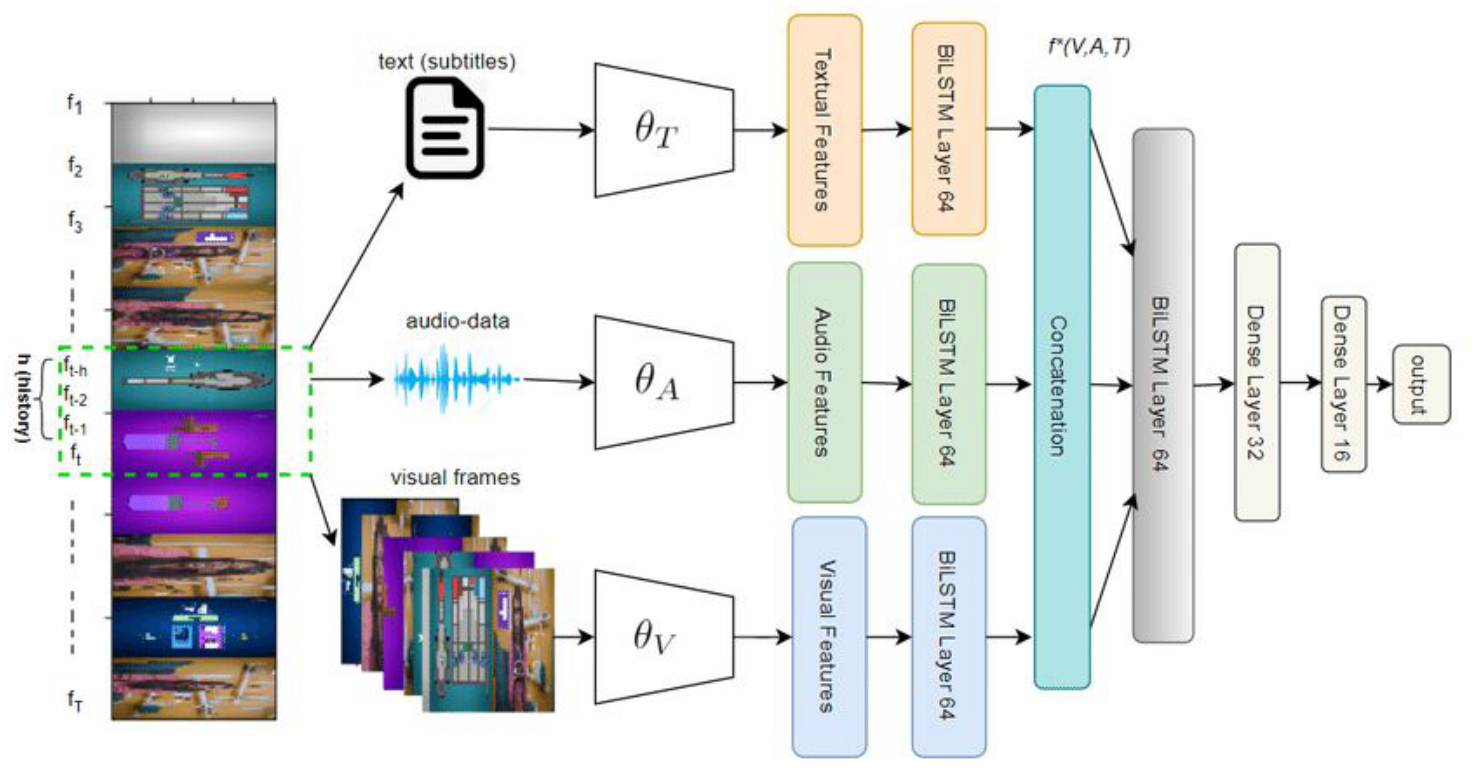
\includegraphics[width=0.8\textwidth, height=0.8\textheight, keepaspectratio]{assets/Lecture-10_Multimodal_NLP_Agentic_AI/slide_023.png}
    \end{column}
  \end{columns}
  \vspace{0.4em}
  \scriptsize
  Adapted from: \textit{Multi-modal Learning for Video Classification} (\href{https://arxiv.org/abs/1904.06409}{arXiv:1904.06409})
\end{frame}

\begin{frame}{Categories of Multimodal Architectures}
  \begin{itemize}
    \item[\textcolor{red}{$\triangleright$}] \textbf{Early Fusion:} Combine raw modalities at the input level.\\
      \textit{Example: VisualBERT adds image embeddings as tokens to the Transformer.}
    \item[\textcolor{red}{$\triangleright$}] \textbf{Late Fusion:} Process each modality separately, then merge representations.\\
      \textit{Example: CLIP encodes images and text independently, then compares embeddings.}
    \item[\textcolor{red}{$\triangleright$}] \textbf{Hybrid / Cross-modal Attention:} Enable interactions between modalities at multiple stages using attention mechanisms.
  \end{itemize}

  \vspace{0.6em}
  \textbf{Design Considerations:}
  \begin{itemize}
    \item[\textcolor{red}{$\triangleright$}] \textbf{Alignment:} How to align representations across modalities.
    \item[\textcolor{red}{$\triangleright$}] \textbf{Modality Dropout:} Handling missing or noisy modalities during training or inference.
    \item[\textcolor{red}{$\triangleright$}] \textbf{Shared vs. Modality-Specific Layers:} Deciding which layers are shared and which are unique to each modality.
  \end{itemize}
\end{frame}

\begin{frame}{Categories of Multimodal Architectures}
  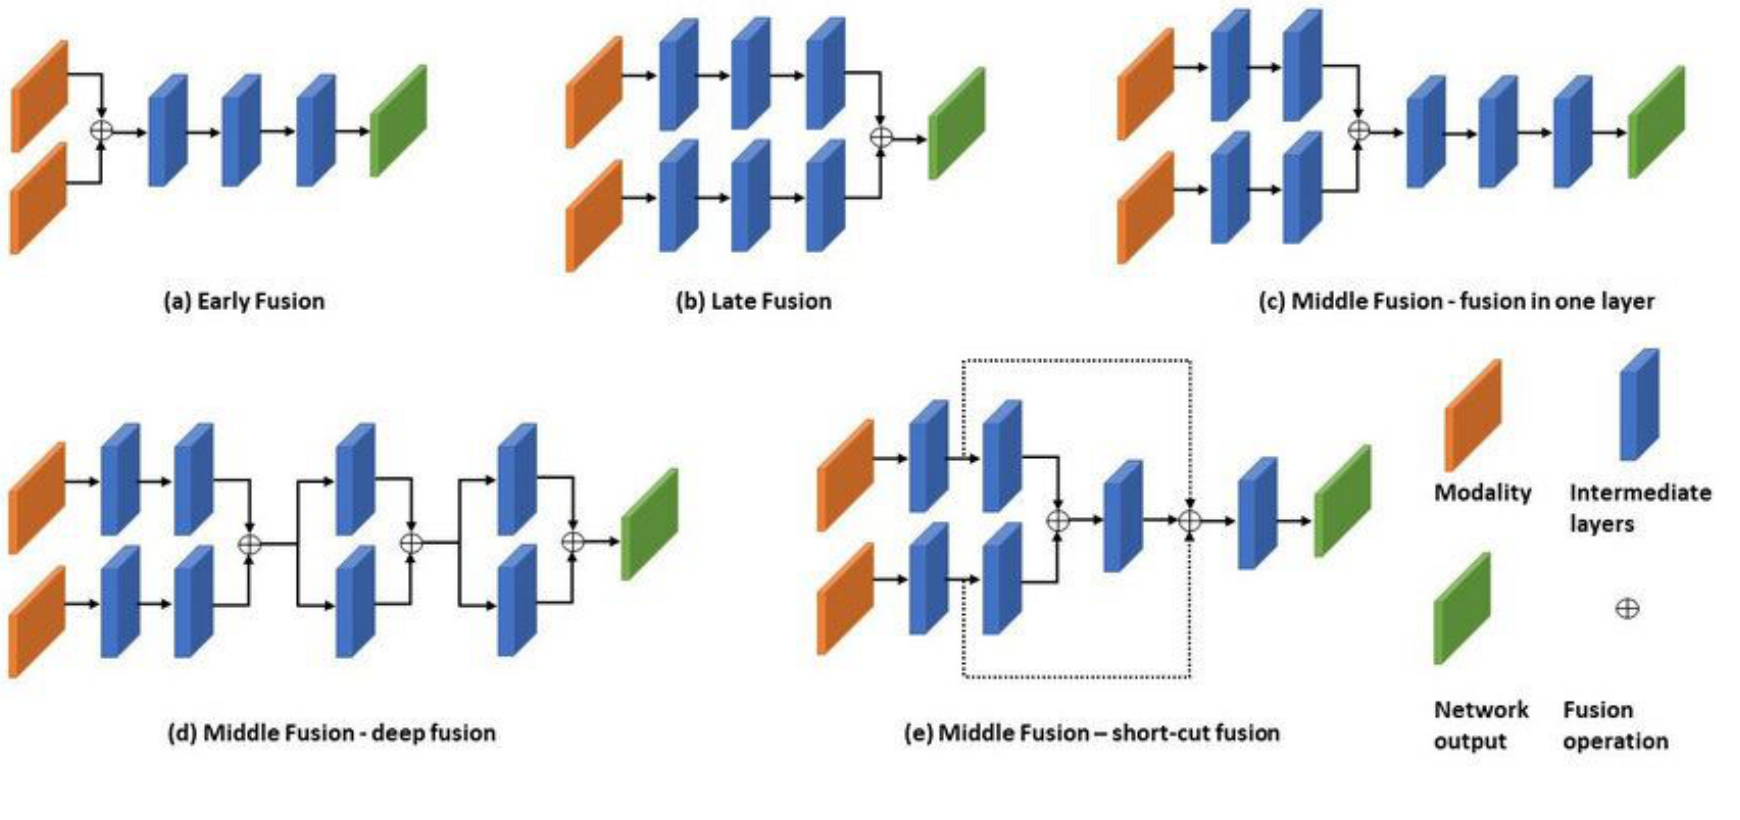
\includegraphics[width=0.98\textwidth, height=0.98\textheight, keepaspectratio]{assets/Lecture-10_Multimodal_NLP_Agentic_AI/slide_025.png}
\end{frame}

\begin{frame}{Early Fusion}
  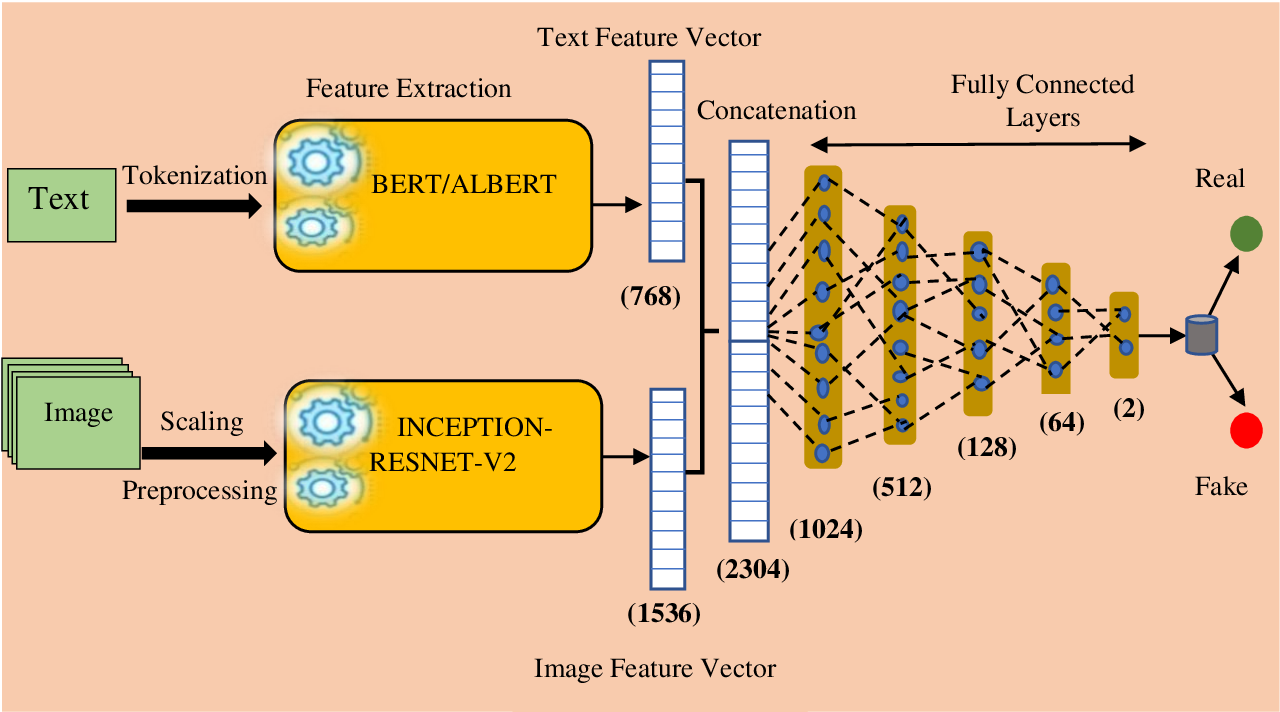
\includegraphics[width=0.98\textwidth, height=0.98\textheight, keepaspectratio]{assets/Lecture-10_Multimodal_NLP_Agentic_AI/slide_026.png}
\end{frame}

\begin{frame}{Late Fusion}
  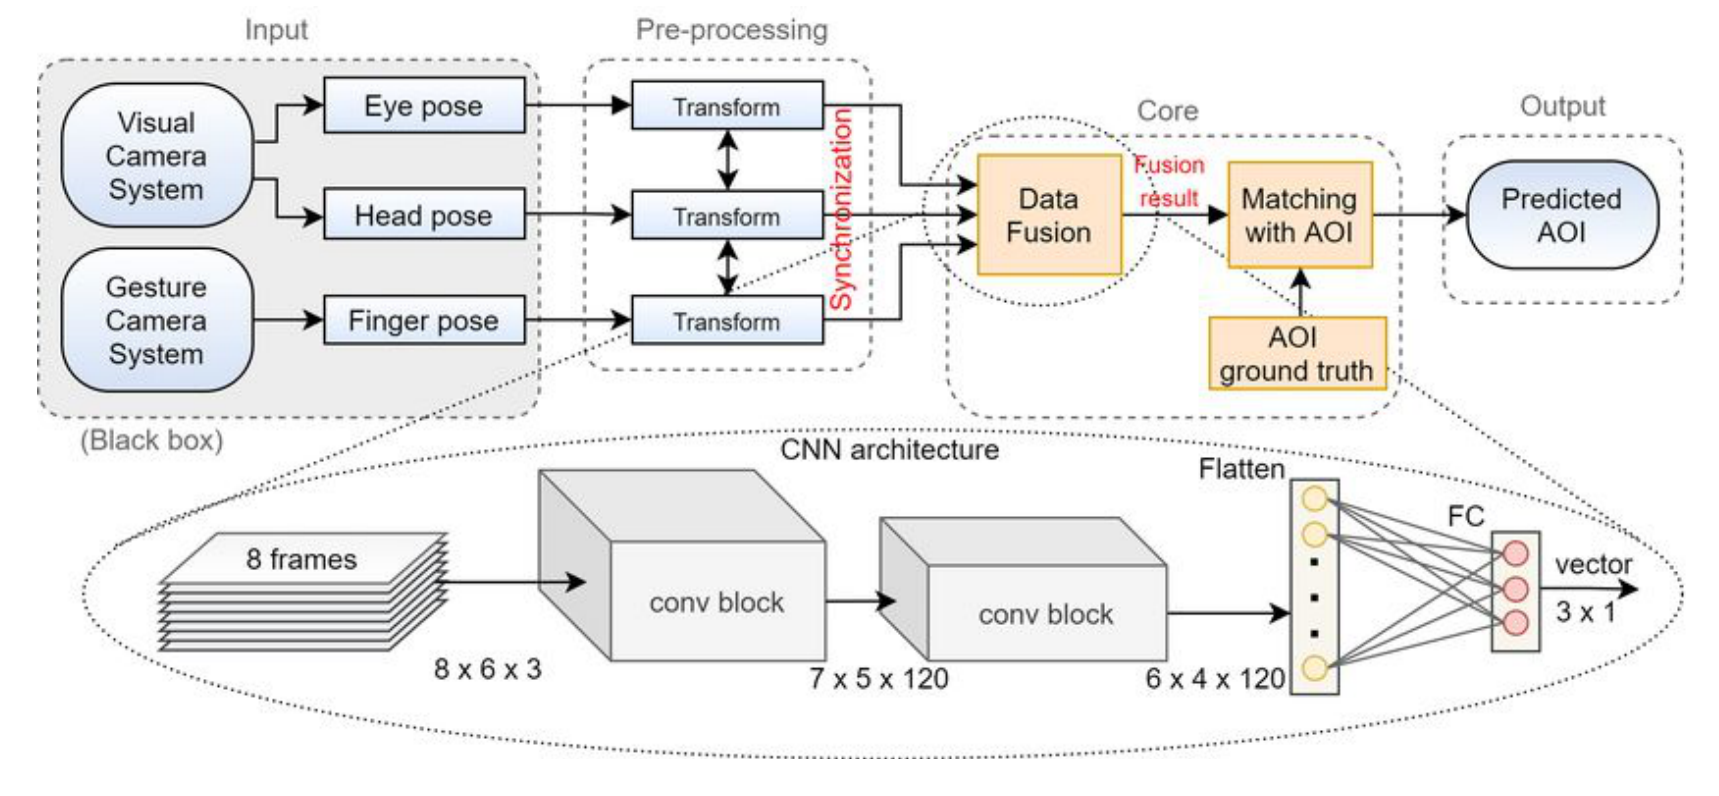
\includegraphics[width=0.98\textwidth, height=0.98\textheight, keepaspectratio]{assets/Lecture-10_Multimodal_NLP_Agentic_AI/slide_027.png}
\end{frame}

\begin{frame}{Challenges in Multimodal Integration}
  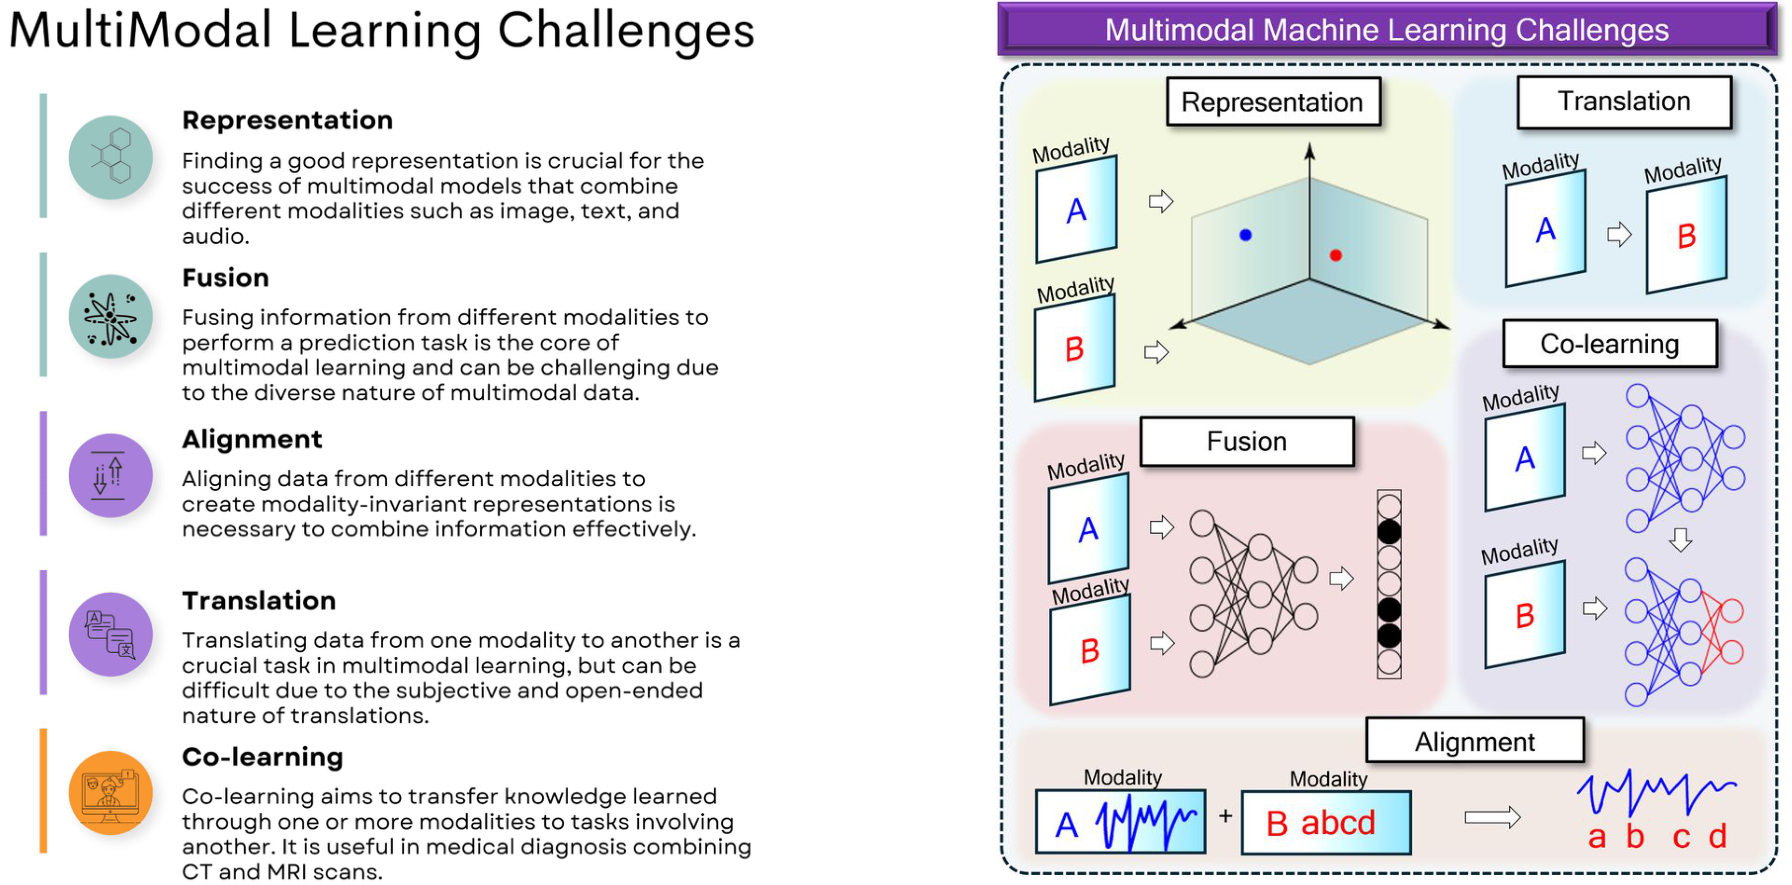
\includegraphics[width=0.98\textwidth, height=0.98\textheight, keepaspectratio]{assets/Lecture-10_Multimodal_NLP_Agentic_AI/slide_028.png}
\end{frame}
